\section{Walidacja}
Przygotowana wersja aplikacji Fokus została udostępniona grupie użytkowników w różnym wieku. Mieli oni za zadanie przetestować funkcje i działanie aplikacji we własnym zakresie. Brak z góry narzuconych scenariuszy testowych oraz kroków do wykonania miał stworzyć warunki naturalnej eksploracji i użycia aplikacji po jej samodzielnym ściągnięciu ze sklepu. Ta decyzja umożliwiła też ocenę bardziej reprezentatywnych statystyk użycia poszczególnych funkcji aplikacji która nie byłaby możliwa w przypadku zastosowania scenariuszy użycia. 

Większość z testerów po raz pierwszy miała styczność z używaną aplikacją co było celowe i miało zwiększyć szansę na uchwycenie wartościowych danych o błędach popełnianych z powodu nieznajomości interfejsu. W miarę jak użytkownicy uczą się nawigacji i elementów aplikacji ich interakcje stają się mechaniczne i nieomylne co zmniejsza prawdopodobieństwo na wyciągnięcie ciekawych wniosków z zebranych danych. Wszystkie dane personalne mogące identyfikować osoby biorące udział w ewaluacji zostały ocenzurowane poprzez ich rozmycie.

\subsection{Powierzchnie interaktywne}
Elementy interfejsu często zawierają wizualnie zaznaczone obszary służące~do~wchodzenia~z~nimi~w~interakcje. Na~poniższym rysunku \ref{fig:interactive_areas} widać dwa przykłady listy elementów~z~których każdy posiada~po~prawej stronie strzałkę. Mając~do~stworzenia tego typu fragment interfejsu pierwszym instynktem może być stworzenie przycisku~ze~strzałką~i~umieszczenie~go~po prawej stronie elementu.

Zebrane interakcje pokazują,~że~pomimo~iż~większość użytkowników instynktownie wybiera właśnie~te~miejsca, część~z~nich dotyka pozostałego obszaru elementu chcąc wykonać~tą~samą akcję. Widoczne~na~prawym obrazku pomarańczowe tło przycisku zastosowane aby przyciągnąć uwagę użytkownika zmniejsza, jednak~nie~pozbywa się zupełnie pozostałych interakcji. 

Powyższe obserwacje wskazują~na~problem~z~opisanym podejściem~do~projektu elementu interfejsu. Brak reakcji aplikacji~na~dotknięcia poza przyciskiem będzie dla użytkowników niezrozumiały~i~frustrujący. Wybrana akcja powinna zostać wykonana~po~dotknięciu dowolnego fragmentu odpowiadającego jej elementu. Powierzchnie interaktywne należy projektować~tak~aby pokrywały możliwie jak największy wizualnie odpowiadający ich akcji obszar ekranu.

\bigskip
\begin{figure}[H]
\centering
\begin{minipage}{.3\textwidth}
	\centering
	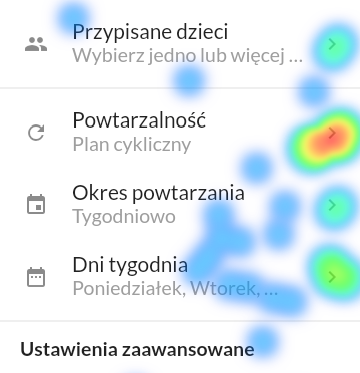
\includegraphics[width=.9\linewidth]{\chapterPath/plan-form.png}
\end{minipage}
\begin{minipage}{.4\textwidth}
	\centering
	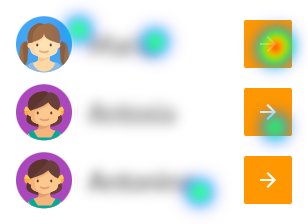
\includegraphics[width=.9\linewidth]{\chapterPath/child-profiles.png}
\end{minipage}
\bigskip
\caption{Przykłady elementów interaktywnych}
\label{fig:interactive_areas}
\end{figure}

\subsection{Problemy użytkowników}
Użytkownicy w naturalny sposób różnią się biegłością w obsłudze urządzeń i aplikacji. Często napotykają oni na tego typu problemy jednak jeśli sami nie poinformują o nich twórców aplikacji ciężko jest im je zidentyfikować. Zwykle tylko marginalny procent użytkowników zadaje sobie trud aby skontaktować się z twórcami i opisać swój problem, dużo częściej ich frustracja rośnie aż do momentu w którym się poddają. Jedyne co w takim przypadku prawdopodobnie zobaczą twórcy (jeśli mają zintegrowane narzędzie monitorujące typu Google Analytics) to kolejny przypadek użytkownika przestającego używać ich aplikacji. 

Narzędzie monitorujące interakcje użytkowników takie jak to stworzone w ramach tej pracy jest w stanie dostarczyć znacznie więcej przydatnych informacji. Dla przykładu rozważmy formularz. Idealną sytuacją która wskazywałaby na brak problemów z jego wypełnieniem byłaby w przybliżeniu jednakowa liczba interakcji z każdym z jego pól oraz końcowym przyciskiem przesyłającym (zakładając że wszystkie pola są obowiązkowe). Taką mapę cieplną można przetłumaczyć jako: ``Wszyscy użytkownicy którzy zaczęli wypełniać formularz zakończyli tą czynność poświęcając przy tym tyle samo uwagi każdemu polu'' (zakładając że uwagę mierzymy w ilości interakcji). 

Na rysunku \ref{fig:pass_issues} widzimy zgoła inną sytuację. Liczba interakcji z kolejnymi polami formularza tworzenia konta w aplikacji znacząco wzrasta, podczas gdy dotknięć przycisku ``Załóż konto'' jest stosunkowo mało. Ponieważ zdecydowana większość użytkowników wypełnia formularze z góry na dół, spadek ilości interakcji z kolejnymi polami jest równoznaczny z zaprzestaniem tej czynności. Sytuacja odwrotna, w której kolejne pola mają zdecydowanie więcej interakcji niż poprzednie może wskazywać na problemy z prawidłowym wypełnieniem przez użytkownika pola posiadającego dodatkową walidację. 

Aplikując powyższe założenia do sytuacji przedstawionej na mapie cieplnej można wywnioskować że niektórzy użytkownicy napotkali na problemy z polem ``Powtórz hasło'' które przypuszczalnie zwracało komunikat o niejednakowych hasłach. Użytkownicy następnie próbowali wielokrotnie wpisywać ponownie hasło w obu polach przypuszczając że się pomylili. Niewiadome jest czy problemy były spowodowane tylko i wyłącznie błędnymi danymi wprowadzanymi przez użytkowników czy też aplikacja działa nieprawidłowo w niewiadomych warunkach, jednak teraz gdy problem został wykryty twórcy mogą zająć się identyfikacją jego dokładnej przyczyny i poprawą działania aplikacji.

\bigskip
\img{\chapterPath/pass-issues.png}{Wypełnianie formularza tworzenia konta}{pass_issues}{.35}

\subsection{Działanie ostrzeżeń}
Ben Schneiderman w znanej książce ``Designing the User Interface: Strategies for Effective Human-Computer Interaction'' \cite{Designing_IU} zaproponował osiem złotych zasad projektowania interfejsów użytkownika. Punkt numer sześć dotyczy umożliwiania łatwego odwrócenia działań mogących mieć niechciane i potencjalnie negatywne dla użytkownika konsekwencje. Kierując się tą zasadą formularze tworzenia planów, nagród oraz odznak w aplikacji Fokus ostrzegają użytkownika o utracie wprowadzonych zmian przy próbie wyjścia z nich. Mapa cieplna okna dialogowego z tym ostrzeżeniem widoczna na rysunku \ref{fig:confirm_warning} potwierdza zasadność reguły Bena Schneidermana. Po przeczytaniu ostrzeżenia większość użytkowników orientuje się że nie chce stracić wprowadzonych zmian i anuluje akcję wyjścia z formularza.

\bigskip
\img{\chapterPath/confirm-warning.png}{Reakcja na ostrzeżenie o utracie danych}{confirm_warning}{.35}

\subsection{Statystyki użycia aplikacji}
Użyteczność narzędzia stworzonego w ramach tej pracy nie ogranicza się tylko i wyłącznie do identyfikacji potencjalnych problemów z interfejsem i weryfikacji wzorców zachowania. Może ono służyć także jako wskaźnik do tworzenia statystyk użycia poszczególnych części i funkcji aplikacji popartych wizualnie sugestywnymi grafikami map cieplnych. Każda grupa elementów interfejsu przedstawiająca dla użytkownika wybór lub będąca jego reprezentacją posiada potencjalną wartość statystyczną dla twórców aplikacji.

Poniżej przedstawione zostały cztery przykłady map cieplnych prezentujących wartość statystyczną w kontekście aplikacji Fokus. Rysunek \ref{fig:star_ratings} przedstawia ekran oceny zadania wykonanego przez dziecko. Opiekun ma możliwość przyznania od jednej do pięciu gwiazdek lub też oznaczenia całego zadania do poprawy. Jak widać ta ostatnia opcja praktycznie nie jest używana a zdecydowana większość ocen to pięć gwiazdek. Stosunkowo często pojawiają się też oceny 4/5 a tylko trzy gwiazdki przyznawane są dosyć rzadko. Takie wykorzystanie funkcji oceny zadań wskazuje na częste zastosowanie pozytywnej afirmacji i powinno być wzięte pod uwagę przy zmianie działania tego elementu w przyszłości.

Na rysunku \ref{fig:signin_methods} przedstawiony jest fragment ekranu logowania użytkowników aplikacji Fokus. Aktualnie użytkownik może wybrać pomiędzy wprowadzaniem standardowej kombinacji adresu mailowego i hasła oraz użyciem konta Google do poświadczenia swojej tożsamości. Pomimo że druga opcja jest znacznie wygodniejsza w użyciu widzimy że użytkownicy korzystają z niej rzadziej.

\bigskip
\begin{figure}[H]
\centering
\begin{minipage}{.45\textwidth}
	\centering
	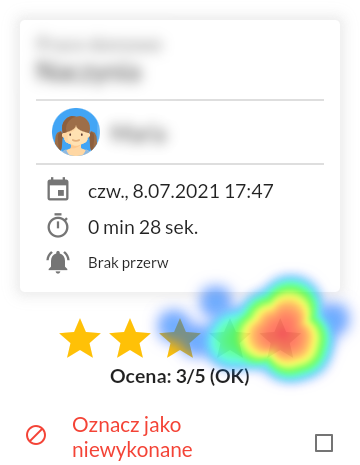
\includegraphics[width=.8\linewidth]{\chapterPath/stars.png}
	\bigskip
	\caption{Ilość gwiazdek przyznawanych przy ocenie zadań}
	\label{fig:star_ratings}
\end{minipage}
\begin{minipage}{.45\textwidth}
	\centering
	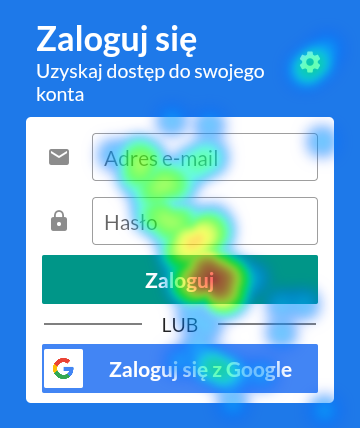
\includegraphics[width=.8\linewidth]{\chapterPath/signin-methods.png}
	\bigskip
	\caption{Preferowane sposoby logowania}
	\label{fig:signin_methods}
\end{minipage}
\end{figure}

Rysunek \ref{fig:plan_length} przedstawia widok listy zadań zawartych w planie. Zadania, przedstawione jako białe karty, mogą reprezentować dowolną wykonywaną przez dziecko czynność. Plan jest zbiorem tematycznie lub czasowo powiązanych ze sobą zadań. Może ich zawierać dowolnie dużo i chociaż na rysunku użyte jest zdjęcie planu z dwoma zadaniami interakcje są zebrane ze wszystkich stworzonych przez testerów planów o potencjalnie różnej długości. Przykładowo, sądząc po wysokości kart, dwie najniżej położone grupy interakcji dotyczą planów o przynajmniej czterech zadaniach. Z rozkładu interakcji zawartych na całej mapie cieplnej łatwo jest stwierdzić że zdecydowana większość tworzonych planów jest dosyć krótkich i zawiera od jednego do trzech zadań (ich karty mają zmienną wysokość i mogą być cieńsze).

Na rysunku \ref{fig:sections_usage} przedstawiony jest dolny pasek nawigacji aplikacji Fokus. Dzieli on ją na trzy główne sekcje: panel z profilami dzieci, zarządzanie planami oraz nagrody i odznaki. Zebranie w całość wszystkich interakcji z kluczowymi elementami nawigacji w formie mapy cieplnej daje dobry wgląd w częstość ich użycia. Widzimy że zdecydowanie najczęściej wykorzystywanym podczas ewaluacji obszarem są plany, co potwierdza ich kluczową dla aplikacji rolę. Najrzadziej otwierana jest zakładka w której tworzone są nagrody i odznaki przyznawane dzieciom. Można to poprzeć faktem że są to dodatkowe funkcje z których można ale nie trzeba korzystać. Mapa cieplna paska nawigacji wykazuje więc że tylko część z użytkowników tworzących plany dodaje też nagrody.

\bigskip
\begin{figure}[H]
\centering
\begin{minipage}{.4\textwidth}
	\centering
	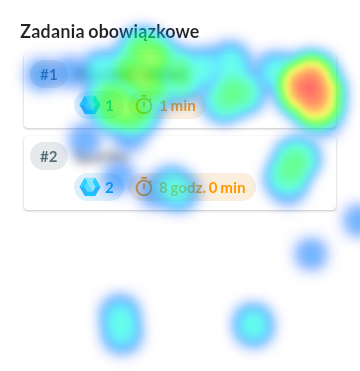
\includegraphics[width=.9\linewidth]{\chapterPath/plan-length.png}
	\bigskip
	\caption{Długość tworzonych planów}
	\label{fig:plan_length}
\end{minipage}
\begin{minipage}{.55\textwidth}
	\centering
	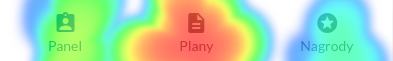
\includegraphics[width=.9\linewidth]{\chapterPath/sections.png}
	\bigskip
	\caption{Częstość użycia głównych sekcji aplikacji}
	\label{fig:sections_usage}
\end{minipage}
\end{figure}

\section{Wnioski}

\subsection{Korzyści} 
Narzędzie pozwala~na~automatyczne zbieranie cennych danych których pozyskanie~w~innym przypadku wymagałyby zorganizowania czasochłonnych testów. Dzięki intuicyjnej, graficznej reprezentacji interakcji połączonej~z~dobrą znajomością interfejsu jego twórca jest~w~stanie znacznie szybciej diagnozować problemy które mają użytkownicy~w~trakcie używania aplikacji. Nagrania kamerą zbierane~z~klasycznych testów~są~zazwyczaj cięższe~i~wolniejsze~w~analizie~z~powodu konieczności manualnego spisywania interakcji, braku informacji~o~dokładnych miejscach dotknięć ekranu oraz częściowym zasłanianiu obrazu~przez~rękę użytkownika. 
